\begin{abstract}
	Language is one of the most important tools that we have. However, we do not always speak the same language, leading to the development of various tools to automatically translate a given language to another language. Neural Machine Translation (NMT) is one of these powerful tools, but it may not cover all terms and vocabulary in various domains. That motivated us to use two different approaches to perform such a task, by implementing an NMT from scratch and fine-tuning an existing model to translate English into Afrikaans using a relatively small data set from an engineering assessment of the Stellenbosch University dataset. We obtained similar performance through these two experiments.
\end{abstract}

\section{Introduction}
Effective communication across languages is crucial in today's globalized world. Machine translation (MT) bridges language barriers by automatically converting text from one language to another. Traditional MT approaches often relied on complex linguistic rules and struggled to capture the nuances of natural language. Neural machine translation (NMT) offers a powerful alternative which leverages deep learning techniques to translate languages directly, achieving higher accuracy and fluency compared to traditional methods. Developing such a model is not easy due to the data requirement and computational cost, so to have insight through them, we will create some simplistic models from scratch and fine-tune an existing model to translate engineering assessments from English to Afrikaans, with a small dataset. For that purpose, we present briefly the basic architecture used in NMT in section \ref{nmt}.  Then, section \ref{mth} focuses on the methodology and finally presents and discusses the result of our experimentation in section \ref{res}.

\section{Neural Machine Translation}\label{nmt}
Translation task consists of converting a text $\mbf{x}=x_{1:T}$ from a language $A$ into a text $\mbf{y}=y_{1:S}$ of a language $B$, that have the same meaning and sense.

Compared to humans, computers do not understand text and even words. But, with the appropriate modelling and tools it can perform such tasks. For Neural Machine Translation (NMT), it assigns a probability  $P_{\mbf{\theta}}(y|x)$ for any possible translation $y$ of $x$ then choose the one with the highest probability. In that case, the probability of the whole translation is given by :
\begin{equation}
	P(\mbf{y}|\mbf{x})=\prod_{t=1}^S P_{\mbf{\theta}}(y_t|y_{1:t-1}, \mbf{x})
\end{equation}
where $\mbf{\theta}$ is the model parameters.
To implement this model, as indicated by the name NMT use a neural network, specifically Encoder-Decoder architecture, illustrated in Figure \ref{fig:enc-dec} and \ref{fig:seq2seq}. In the Encoder part, the input is compressed into a smaller representation, which is fed into the Decoder part to produce an input with a specific target.
\begin{figure}[H]
	\centering
	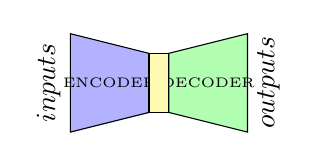
\begin{tikzpicture}
		\draw[fill=blue!30]  (0,0) -- (1, -0.25) -- (1, -1) -- (0,-1.25) -- cycle node[midway, left] {\rotatebox{90}{$\mbf{inputs}$}};
		\node[font=\tiny](enc) at (0.5, -0.62) {ENCODER};


		\draw[fill=green!30]  (1.25,-0.25) -- (2.25, 0) -- (2.25, -1.25) node[midway, right] {\rotatebox{90}{$\mbf{outputs}$}}-- (1.25,-1) -- cycle;
		\node[font=\tiny](enc) at (1.75, -0.62) {DECODER};
		\draw[fill=yellow!30] (1, -.25) rectangle  (1.25, -1);
	\end{tikzpicture}
	\caption{Illustration of an encoder-decoder architecture}
	\label{fig:enc-dec}
\end{figure}
Treating, text data as a sequence, we use Recurrent Neural Networks (RNNs, Figure \ref{fig:rnn}), which predict a single word at a time, and the model is often called seq2seq (sequence-to-sequence) model. Recurrent neurons depend on their previous outputs or states, which is the property that differentiates them from classical neurons.
\begin{figure}[H]
	\centering
	\begin{subfigure}{0.2\linewidth}
		\scalebox{0.75}{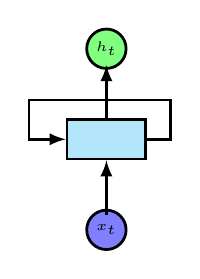
\begin{tikzpicture}
				\draw[line width=1pt, fill=blue!50] (0,-1.15) circle (0.25);
				\draw[line width=1pt, fill=green!50] (0,1.15) circle (0.25);
				\node[font=\tiny] (x) at (0, -1.15) {$\mbf{x_t}$};
				\node[font=\tiny] (h) at(0, 1.15) {$\mbf{h_t}$};
				\node[draw, rectangle, minimum height=0.5cm, minimum width=1cm, line width=1pt, fill=cyan!30] (a) at (0,0) {};
				\draw[->,>=latex, line width=1pt] (x.north)--(a);
				\draw[->,>=latex, line width=1pt] (a)--(h);
				\draw[line width=1pt,->, >=latex] (a.east) --++(0.3, 0) --++(0, 0.5) --++(-1.8,0) --++(0, -0.5) -- (a.west);
		\end{tikzpicture}}
		\caption{An RNN}
		\label{fig:rnn}
	\end{subfigure}\begin{subfigure}{0.8\linewidth}
		\scalebox{0.75}{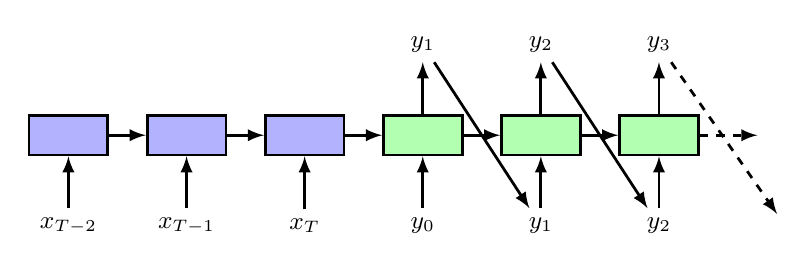
\begin{tikzpicture}
				\begin{scope}
					\node[font=\small] (x) at (0, -1.15) {$\mbf{x_{T-2}}$};
					\node[draw, rectangle, minimum height=0.5cm, minimum width=1cm, line width=1pt, fill=blue!30] (e1) at (0,0) {};
					\draw[->,>=latex, line width=1pt] (x)--(e1);
				\end{scope}
				\begin{scope}[xshift=1.5cm]
					\node[font=\small] (x) at (0, -1.15) {$\mbf{x_{T-1}}$};
					\node[draw, rectangle, minimum height=0.5cm, minimum width=1cm, line width=1pt, fill=blue!30] (e2) at (0,0) {};
					\draw[->,>=latex, line width=1pt] (x)--(e2);
				\end{scope}
				\begin{scope}[xshift=3cm]
					\node[font=\small] (x) at (0, -1.15) {$\mbf{x_T}$};
					\node[draw, rectangle, minimum height=0.5cm, minimum width=1cm, line width=1pt, fill=blue!30] (e3) at (0,0) {};
					\draw[->,>=latex, line width=1pt] (x)--(e3);
				\end{scope}

				%%%%%%%%%%%%%%%%%%%%%%%%%%%
				\begin{scope}[xshift=4.5cm]
					\node[font=\small] (x1) at (0, -1.15) {$\mbf{y_0}$};
					\node[font=\small] (y1) at (0, 1.15) {$\mbf{y_1}$};
					\node[draw, rectangle, minimum height=0.5cm, minimum width=1cm, line width=1pt, fill=green!30] (d1) at (0,0) {};
					\draw[->,>=latex, line width=1pt] (x1)--(d1);
					\draw[->,>=latex, line width=1pt] (d1)--(y1);
				\end{scope}
				\begin{scope}[xshift=6cm]
					\node[font=\small] (x2) at (0, -1.15) {$\mbf{y_1}$};
					\node[font=\small] (y2) at (0, 1.15) {$\mbf{y_2}$};
					\node[draw, rectangle, minimum height=0.5cm, minimum width=1cm, line width=1pt, fill=green!30] (d2) at (0,0) {};
					\draw[->,>=latex, line width=1pt] (x2)--(d2);
					\draw[->,>=latex, line width=1pt] (d2)--(y2);
				\end{scope}
				\begin{scope}[xshift=7.5cm]
					\node[font=\small] (x3) at (0, -1.15) {$\mbf{y_2}$};
					\node[font=\small] (y3) at (0, 1.15) {$\mbf{y_3}$};
					\node[draw, rectangle, minimum height=0.5cm, minimum width=1cm, line width=1pt, fill=green!30] (d3) at (0,0) {};
					\draw[->,>=latex, line width=1pt] (x3)--(d3);
					\draw[->,>=latex, line width=1pt] (d3)--(y3);
				\end{scope}


				\draw[->,>=latex, line width=1pt] (e1)--(e2);
				\draw[->,>=latex, line width=1pt] (e2)--(e3);
				\draw[->,>=latex, line width=1pt] (e3)-- (d1);
				\draw[->,>=latex, line width=1pt] (d1)--(d2);
				\draw[->,>=latex, line width=1pt] (d2)--(d3);
				\draw[->,>=latex, line width=1pt, dashed] (d3)-- ++(1.25, 0);

				\draw[->,>=latex, line width=1pt] (y1)--(x2);
				\draw[->,>=latex, line width=1pt] (y2)--(x3);
				\draw[->,>=latex, line width=1pt, dashed] (y3)--(9, -1.);
		\end{tikzpicture}}
		\caption{A seq2seq model}
		\label{fig:seq2seq}
	\end{subfigure}
	\caption{RNN and Encoder-Decoder architecture}
\end{figure}

The major problem of the basics of the RNNs is the vanishing and exploding gradient. This is solved by using more advanced architecture like Gated Recurrent Unit (GRU), and Long Short-Term Memory (LSTM).
However, these architectures can be hard to train and computationally slow due to their recurrence. In addition, these models may perform poorly when dealing with long sequences.

Inspired by how humans translate a sentence, researchers introduce attention mechanisms. This technique allows the model to keep track of the long-term dependency, and not rely only on the compressed version from the encoder, but with the output of the encoder at each time step.

Furthermore, they come up with the self-attention mechanism by producing the layer  $n$ as a form of the weighted sum of the previous layer $n-1$. This method does not need any more recurrency between each term of the sequence. Lastly, attention and self-attention are the main components of the so-called transformer block found at the state-of-the-art of many machine learning models today.


The optimal weights of the neural networks (parameters) $\mbf{\theta}$ are found by minimizing the per-word (sequence) negative log-likelihood:
\begin{equation}
	J(\mbf{\theta}) = -\frac{1}{S}\sum_{i=1}^{S}\log P_{\mbf{\theta}}(y_t|y_{1:t-1}, \mbf{x})
\end{equation}
Which can be done by using gradient-based optimisation.

\section{Methodology}\label{mth}
This section presents different parts of the methodology in our experimentation and the reasons behind them.

\subsection{Dataset}
The initial dataset is a relatively small parallel English-Afrikaans from an engineering assessment of Stellenbosch University. This dataset is then augmented with data from Tatoeba \cite{tatoeba}. As the assessment comes from \LaTeX files, we combine all the mathematical environments by removing spaces to treat them as a single word. We also add space on delimiter characters such as ``(),[],\{\}'' to treat them as a single word by removing extra spaces. Finally, we switched it to lowercase to be more efficient for our from-scratch implementation, and a special character token for the start of the sentence and the end of the sentence is used to replace ``!, ? and .'' in the text.


But, in the second part of the experimentation, we just handled the latex mathematical environment without changing the case and used the tokenizer provided by the pre-trained model that we used.

\subsection{From Scratch Implementation}

We principally focus on the fundamental basis of the implementation with PyTorch, so we use the same hyper-parameter for each implemented model as in Table \ref{tab:hyper}.
\begin{table}[H]
	\centering
	\begin{tabular}{lc}
		\toprule
		Parameter & Value \\
		\midrule
		Embedding Size & 256 \\
		Hidden Size & 1024 \\
		Number of Layers & 2 \\
		\bottomrule
	\end{tabular}
	\caption{Hyperparameters used in the from-scratch models.}
	\label{tab:hyper}
\end{table}
Thus, with these parameters, we implement the following model:
\begin{itemize}
	\item Vanilla: RNNs, GRU, LSTM
	\item With scaled dot-product attention:  RNNs, GRU, LSTM
\end{itemize}
The scaled dot product is defined is defined by :
\begin{equation}
	a(\mbf{q, v}) = \frac{\mbf{q^\top v}}{\sqrt{D}}
\end{equation}
where $\mbf{q}$ is the current output of the decoder, $\mbf{v}$ an output of the decoder at some time step, and  $D$ is the dimension of $\mbf{q}$ (and $\mbf{v}$ as well because they must have the same dimension).These value are passed through a $\softmax$ layer to have a vector formed by some $\alpha[0,1]$, then we compute the context vector given by :
\begin{equation}
	\mbf{c}_s = \sum_{i=1}^{T}\alpha_i \mbf{v}_i
\end{equation}
This later is then concatenated with $\mbf{q}_s$ to produce the final output of the decoder at step $s$.

Finally, we train each model with at most $50$ epochs, using the NAdam optimizer with $10^{-3}$ as the learning rate. Note that we did not perform any explicit hyperparameter tuning for these models. We use a sentence to observe the evolution of the model during training and stop it once it has output a perfect prediction, or there is no more evolution in the loss value during training (manually ...). This is done to avoid over-fitting on the training set.

\subsection{Using a Pre-trained Model}
A pre-trained model is a model which is already trained on some data set for a specific task. So, Leveraging such a model can be a highly efficient approach, and allows us to save substantial time and resources. Usually trained on massive amounts of data, therefore it contains already an important amount of information.

For this task, we will perform a fine-tuning, e.g., we will re-train the model on our dataset to give the model a more specific domain and vocabulary as it may have not seen data such as engineering assessment. This practice is also known as domain shifting.

Since we aim to translate English to Afrikaans, we fine-tune the \texttt{opus-mt-en-af} model which can already perform the given task but has not yet adapted to our requirement. Based on the Marian-MT framework \cite{marian}, this model is part of a larger collection of open-source high-performant Neural Machine Translation (NMT) models \cite{OPUSMT}.

The opus-mt-en-af model was initially trained on a public dataset from the Open Parallel Corpora \cite{opus}, which contains a strong foundation. However, it may not contain some specific vocabulary from the engineering domain. Thus by fine-tuning the model on our dataset, we expect to improve its performance in handling these specialized terms and phrases. Here we only use the engineering assessment data set because the Tatoeba data set is part of the training data of the model.

To implement this task, we use the \texttt{transformer} library that allows us to obtain the weights of the model from Hugging Face \cite{huggingface} using PyTorch. It also allows us to tokenize our data set, using the tokenized provided by opus-mt which is based on \texttt{sentencepiece} \cite{sentencepiece} of Google (with the de-tokenizer as well).

For the parameter optimization of the model, AdamW  \cite{AdamW} as suggested in the Hugging Face NLP course for the translation model fine-tuning.

\subsection{Model evaluation}
We evaluate all the models by computing the bilingual evaluation understudy (BLEU) metric. It measures how similar the results of the machine translation are to human translation (references).

For the from-scratch implementation, we evaluate the augmented dataset and the engineering assessment only.

For the fine-tuning, we evaluate it before the training and after training on the validation set, this is done to see if we are effectively able to improve the model on the new domain.


\section{Results and Discussion}\label{res}
After training our model, we present in this section the results and discussion related to our experimentation.

\subsection{From-Scratch Implementation}
Figure \ref{fig:loss1} shows the loss per epoch for each model. We stopped the training at specific epochs to avoid over-fitting on the training set once we had several epochs where the model predicted our monitoring sentence perfectly. We also note that we did not perform any hyperparameter tuning.

\begin{figure}[H]
	\centering
	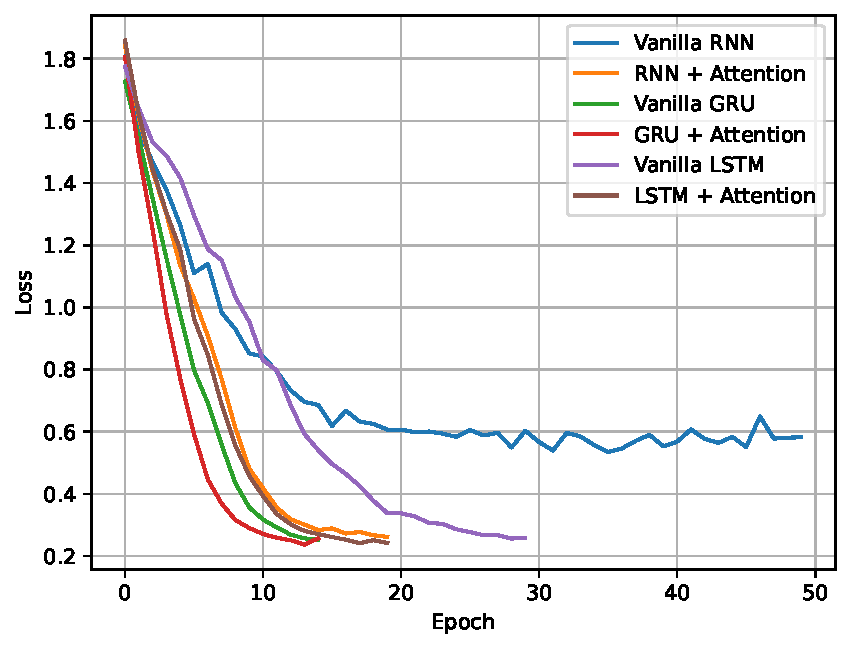
\includegraphics[width=0.9\linewidth]{./figures/vanilla.pdf}
	\caption{Epoch/Loss for from-scratch implementation}
	\label{fig:loss1}
\end{figure}

As we can observe, the vanilla RNN got stuck during the training process, which is confirmed in Table \ref{tab:tab1}, but it may be improved by adjusting some of the hyper-parameter of the model we did not do that. However, it drastically improved.

On the other hand, the other model converges quickly into an optimal parameter.

\begin{table}[H]
	\centering
	\begin{tabular}{lccccc}
		\cmidrule(l){3-6}
		\multicolumn{2}{l}{} & \multicolumn{2}{c}{Validation Set 1} & \multicolumn{2}{c}{Validation Set 2} \\ \midrule
		Model     & \#Epochs & BLEU G          & BLEU B         & BLEU G          & BLEU B         \\ \midrule
		RNN       & 50       & 0.07            & 0.05           & 0.10            & 0.08           \\
		GRU       & 15       & 0.38            & 0.36           & 0.15            & 0.12           \\
		LSTM      & 30       & 0.34            & 0.33           & 0.14            & 0.13           \\
		RNN+Att.  & 20       & 0.37            & 0.33           & 0.17            & 0.17           \\
		GRU+Att.  & 15       & 0.30            & 0.33           & 0.12            & 0.14           \\
		LSTM+Att. & 20       & 0.30            & 0.29           & 0.12            & 0.13           \\ \bottomrule
	\end{tabular}
	\caption{BLEU scores for each from-scratch model on the validation set}
	\label{tab:tab1}
\end{table}

Table \ref{tab:tab1} provides the BLEU scores for each model on augmented Validation Set 1 and the original Validation Set 2. We also used to approach to generate the prediction. Greedy search (G) and beam search of width 3 (B).

We also observe a huge difference between the Vanilla RNNs and the RNNs with Attention, while the performance of other models dropped with the attention mechanism.

However, using an attention mechanism stabilizes the model training, thus these performances can be improved through some hyper-parameter tuning.

Using these models we have for example ``motivate your answer'', is translated into ``motiveer jou'',  where the reference ise ``motiveer jou antwoord''. This is the only which appears good from the example that we printed out \footnote{We can see more examples in the notebook}.


Now let us have a look at the result from the fine-tuned model.

\subsection{Fine-Tuning}
The \texttt{opus-mt-en-af} seems to respond well to the new data set as shown in Figure \ref{fig:loss2}.
\begin{figure}[H]
	\centering
	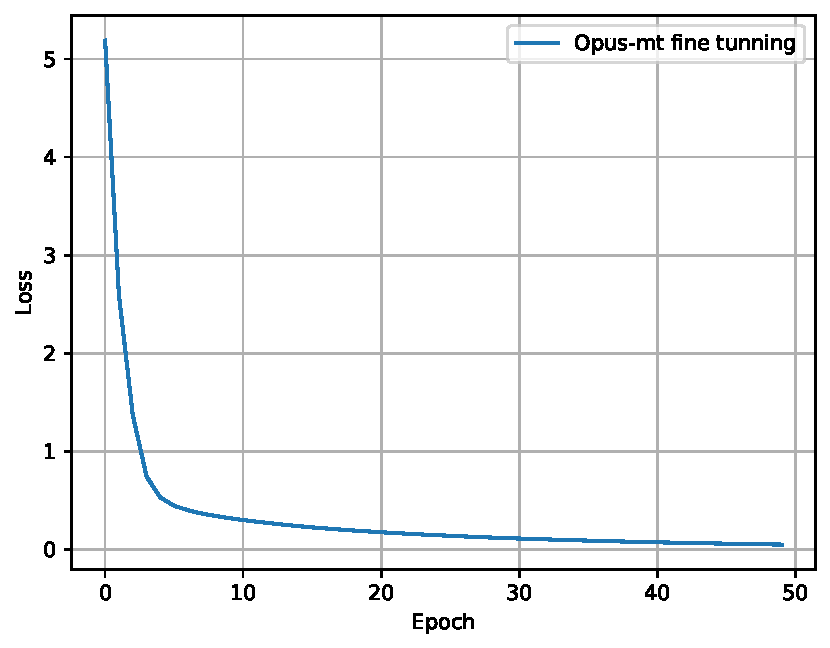
\includegraphics[width=0.8\linewidth]{./figures/fine_tunning.pdf}
	\caption{Epoch/Loss for fine-tuning implementation}
	\label{fig:loss2}
\end{figure}

As we measured the BLEU score on the validation set before and after training, Table \ref{tab:fine} shows that the model was able to learn new things from the data set passing from a BLEU of 0.28 to 0.37, after training it for 50 epochs with a learning rate of $2\times 10 ^{-5}$.

\begin{table}
	\centering
	\begin{tabular}{lccc}
		\toprule
		Model                 & \#Epochs & LR              & BLEU \\
		\midrule
		opus-mt-en-af         & N/A      & N/A             & 0.28 \\
		Fine-tuned opus-mt-en-af & 50      & $2\times10^{-5}$ & 0.37 \\
		\bottomrule
	\end{tabular}
	\caption{BLEU score of the original and fine-tuned opus-mt model on the validation set}
	\label{tab:fine}
\end{table}
Overall,  fine-tuning a model is beneficial when we have a small dataset, and it proved a more handy and better implementation by avoiding re-inventing things that already exist. We can see some examples of translation in Figure \ref{fig:example}.

\begin{figure}[H]
	\centering
	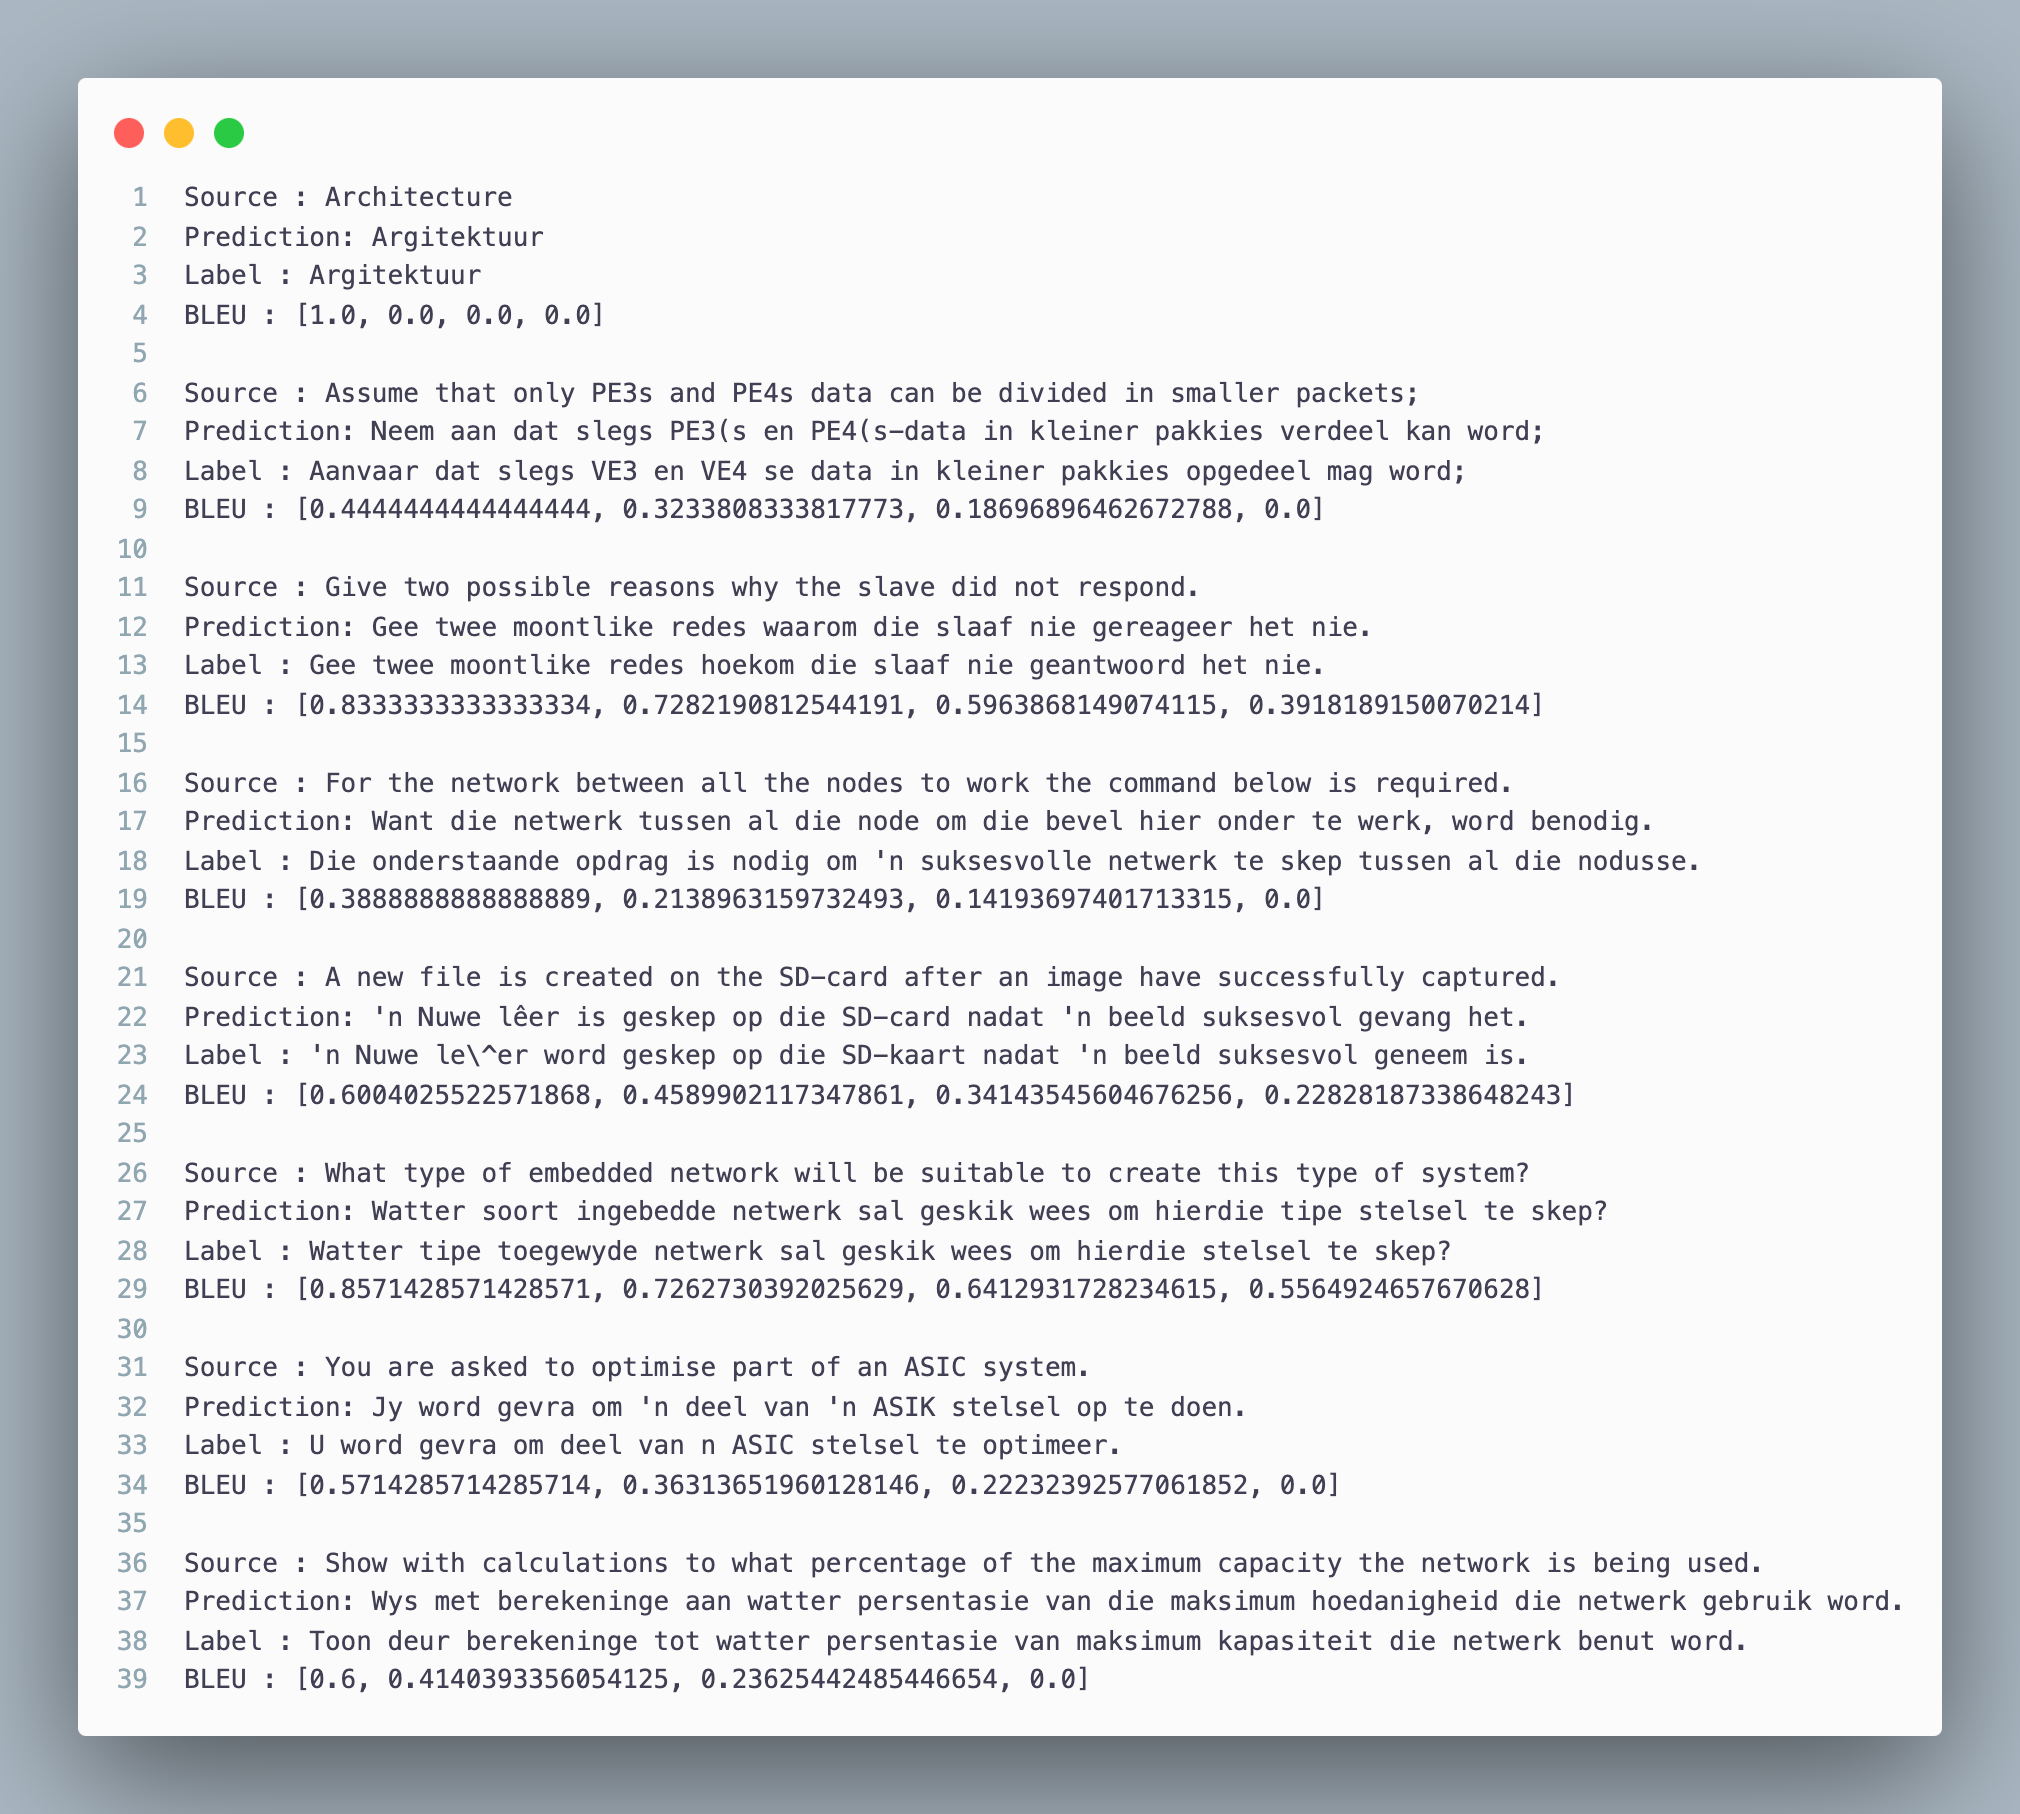
\includegraphics[width=\linewidth]{./figures/example.png}
	\caption{Examples of translation from the fine-tuned Model}
	\label{fig:example}
\end{figure}



\subsection{General discussion between the two approaches}
Comparing the from-scratch models and the fine-tuned models, several points emerge:
\begin{itemize}
	\item Training Efficiency: The from-scratch models required careful monitoring to avoid over-fitting, hyper-parameter tuning, and architecture choice which may require huge computation resources depending on architecture and dataset. In contrast, fine-tuning a pre-trained model was more efficient and resulted in better performance by leveraging the existing functionality.

	\item Model Performance: The best from-scratch model (GRU/RNN+Att) achieved a BLEU score of 0.38/0.37, which is close to the fine-tuned model's score of 0.37. This demonstrates that while from-scratch models can achieve competitive performance, but may require a bigger effort.
\end{itemize}

An important thing to mention is the dataset, to develop a domain-specific machine translation, it is always better to gather as much as possible the model some data from the domain of interest. Otherwise will spend a lot of time tuning and training it to obtain a poor performance at the end.


\section{Conclusion}
In conclusion, we have explored the basis of Neural Machine translation and learned how to implement the vanilla RNN, GRU, and LSTM including a version with an attention mechanism, using PyTorch to translate English to Afrikaans. We also fine-tuned the ``\texttt{opus-mt-en-af}'' to perform the same task. Our best model GRU from scratch achieved a BLEU score of 0.38 on the augment data set while the fine-tuned model achieved 0.37. We also encounter the importance of the training data to obtain a translation of quality. The future perspective is to improve the coding styles and architecture to have a useful code base and try other tokenization approaches as well as hyper-parameter tuning.

\begin{thebibliography}{1}

	\bibitem{kamper2022nlp817} Herman Kamper. \emph{NLP817}. \href{https://www.kamperh.com/nlp817/}{https://www.kamperh.com/nlp817/}, 2022--2024.
	\bibitem{huggingface} Hugging Face \href{https://huggingface.co/}{https://huggingface.co/}
	\bibitem{tatoeba} Tatoeba \href{https://tatoeba.org/en}{https://tatoeba.org/en}, 16/07/2024.
	\bibitem{opus} Open Parallel Corpora \href{https://opus.nlpl.eu/}{https://opus.nlpl.eu/}
	\bibitem{AdamW} AdamW \href{https://pytorch.org/docs/stable/generated/torch.optim.AdamW.html}{https://pytorch.org/docs/stable/generated/torch.optim.AdamW.html}
	\bibitem{sentencepiece} Sentencepiece \href{https://github.com/google/sentencepiece}{https://github.com/google/sentencepiece}
	\bibitem{helsinki} Helsinki NLP \href{https://blogs.helsinki.fi/language-technology/}{https://blogs.helsinki.fi/language-technology/}, \href{https://huggingface.co/Helsinki-NLP}{https://huggingface.co/Helsinki-NLP}
	\bibitem{marian} Junczys-Dowmunt, M., Grundkiewicz, R., Dwojak, T., Hoang, H., Heafield, K., Neckermann, T., Seide, F., Germann, U., Aji, A.F., Bogoychev, N. and Martins, A.F., 2018. Marian: Fast neural machine translation in C++. \textit{arXiv preprint arXiv:1804.00344.}
	\bibitem{OPUSMT} Jörg Tiedemann and Santhosh Thottingal. 2020. OPUS-MT - Building open translation services for the World. \textit{In Proceedings of the 22nd Annual Conference of the European Association for Machine Translation, pages 479–480, Lisboa, Portugal. European Association for Machine Translation.}
\end{thebibliography}